\section{Redes de Sensores Sem Fio}
	\cite{Silva2009}
	Com a queda crescente nos custos dos equipamentos eletr�nicos, a redu��o no tamanho dos dispositivos simplificando a sua mobilidade, fez com que as redes sem fio ganhassem popularidade rapidamente mundo afora, ganhando novos tipos de aplica��es com objetivo de simplificar o dia-a-dia das pessoas, como previsto por Weiser em \cite{Weiser1991}. 

	Atualmente, a variedade de sensores\cite{SensoresXXXX} existentes e que podem ser obtidos sem muita dificuldade pela internet tem crescido exponencialmente. Aliado � uma consci�ncia dos benef�cios que a interliga��o desses dispositivos em rede para an�lise em tempo real das informa��es ambientais, geralmente invis�veis a nossa aten��o no curto prazo \cite{Weiser:1997:CAC:504928.504934} podem oferecer ao dia-a-dia, faz da rede de sensores sem fio um dos pilares de sustenta��o da Internet das Coisas (IoT).

	Decis�es sobre a arquitetura, modelo e equipamentos utilizados em uma Redes de Sensores Sem Fio \cite{LECKER2010} (RSSF ou WSN) se tornaram fator de sucesso para projetos de IoT.

\begin{figure}[tbh!]
	\centering
	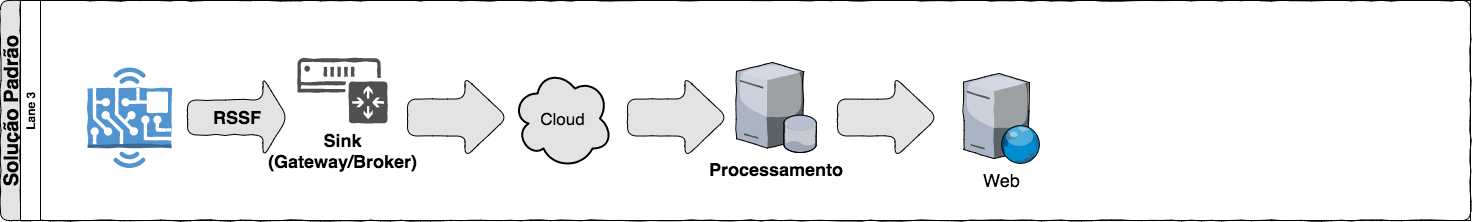
\includegraphics[width=1.0\textwidth]{../images/padrao_rede}
	\caption{Arquitetura RSSF padr�o}
	\label{fig:rssfpadrao}
\end{figure}

Em \cite{Ueyama002840382} e \cite{Furquim002744726}, uma estrutura de sensores do tipo b\'{o}ia foi criada para coleta e an�lise do n�vel da �gua e sua polui��o em rios.

\begin{figure}[tbh!]
	\centering
	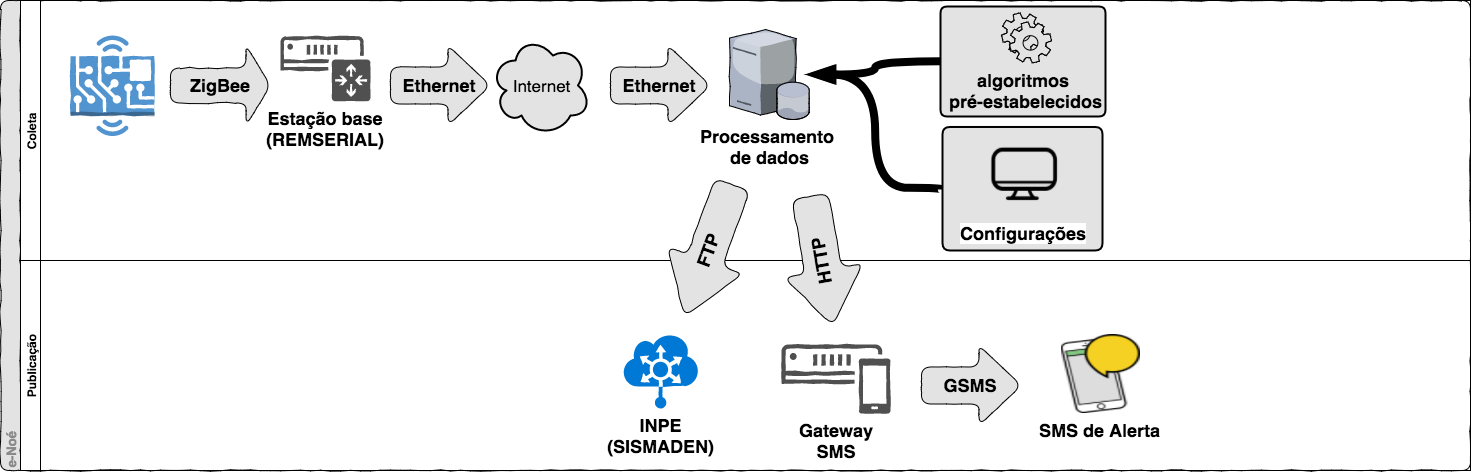
\includegraphics[width=1.0\textwidth]{../images/enoe_rede}
	\caption{Projeto e-No�}
	\label{fig:enoe}
\end{figure}

De acordo com o trabalho realizado em \cite{Chen2014}, podemos analisar, classificar e quantificar os insetos encontrados em uma determinada regi�o utilizando sensores ac�sticos, de forma a utilizar os resultados encontrados para aplica��o de uma quantidade determinada de defencivos, controlando o efeito de sua aplica��o em tempo real.

Para se criar um modelo automatizado para controle do uso de recursos com custos reduzidos de forma a gerar menor impacto financeiro aos agricultores familiares � imprecindivel se  

Na pr�tica seria usar RSSF, sensores, atuadores e um sistemas distribu�do para automatizar processos como o de gotejamento localizado como descrito nas imagens abaixo, baseado em informa��es retiradas da bdpa (base de pesquisas agropecu�ria) da embrapa.